\section{Introduction}
\lipsum[1]

\subsection{Prior Literature}

As discussed in \cite{Eyer2010a,Sioshansi2012,Denholm2013,Makarov2012}, the findings from \cite{Walawalkar2007,Sioshansi2009} are clearly refuted. 
\lipsum[66]

This is in contrast with the methods of \cite{Kazempour2009,Kirby2012}, and the conventional modeling of \cite{EnergyandEnvironmentalEconomicsE32014a,Eyer2010a,Dunn2011,DepartmentofEnergy}. \lipsum[55]

%%%%%%%%%% SECTION

\section{Formulation}

\lipsum[5]

\begin{tabular}{c l}
$k$ 					& Time index, from 0 to time horizon $N$ \\
$\Delta t$ 				& Time step size (hours) \\
$c(k)$					& Energy flow into the battery at time $k$ (kW) \\
$d(k)$					& Energy flow out of the battery at time $k$ (kW) \\
$\text{P}_{\text{charge}}$		& Maximum charge power capacity of the system (kW) \\
$\text{P}_{\text{discharge}}$	& Maximum discharge power capacity of the system (kW) \\
$\text{c}_{\text{grid}}(k)$	& Nodal electricity clearing price (\$/kWh) \\
$\text{\texteta}_{\text{in}}$		& One-way system efficiency when charging \\ 
$\text{\texteta}_{\text{out}}$		& One-way system efficiency when discharging \\
$E(k)$					& Energy level in reservoir at time k \\
$\text{E}_{\min}$				& Minimum allowable energy level as portion of capacity \\
$\text{E}_{\max}$				& Maximum allowable energy level as portion of capacity \\
$\text{E}_{\text{init}}$		& Starting energy level of the storage system \\
$h$						& Reservoir capacity (h), in hours of peak discharge \\
$\text{\textgamma}$				& Annualized cost of constructing one kWh of reservoir capacity (\$/kWh/yr)
\end{tabular}


\subsection{Data}
\lipsum[2] As clearly demonstrated in Figure \ref{fig:datamap}

\begin{figure}
\centering
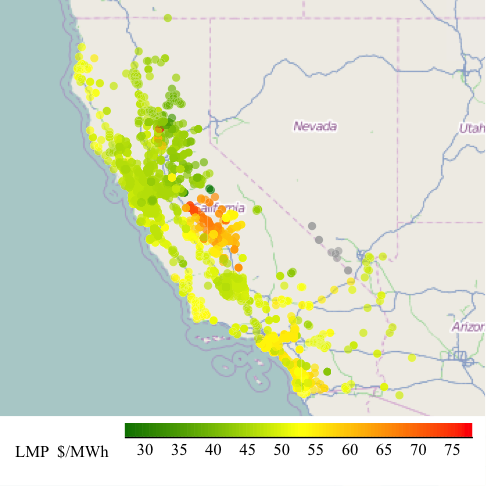
\includegraphics[trim = 0mm 0mm 0mm 0mm, clip, width=0.6\textwidth]{Figures/unprocessed_LMP_map.png}
\caption{Example of Location Marginal Price (LMP) distribution on the CAISO grid. Each circle represents an LMP node on the the CAISO grid. Data from 4PM PDT, August 18 2013}
\label{fig:datamap}
\end{figure}

\section{Results}
In Fig. \ref{fig:chargesize}, \lipsum[66]

\begin{figure}
\centering
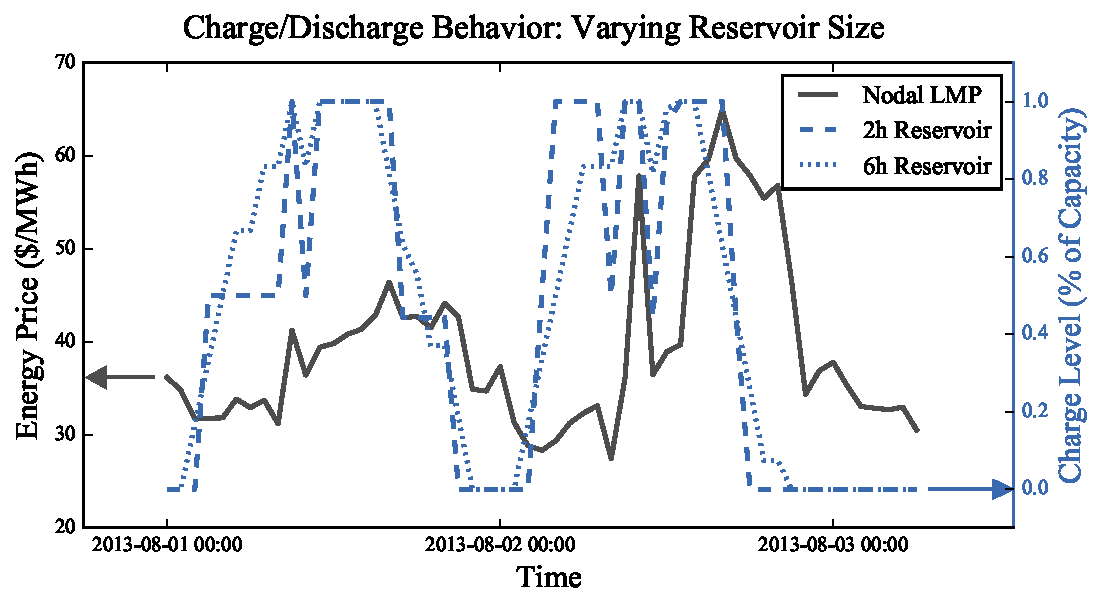
\includegraphics[trim = 0mm 0mm 0mm 0mm, clip, width=0.8\textwidth]{Figures/chargeValidation_varyingSize}
\caption{ Aenean massa. Cum sociis natoque penatibus et magnis dis parturient montes, nascetur ridiculus mus. Donec quam felis, ultricies nec, pellentesque eu, pretium quis, sem. Nulla consequat massa quis enim. }
\label{fig:chargesize}
\end{figure}

\lipsum[2-3]

%%%%%%%%%% CONCLUSION

\section{Conclusion}
\lipsum[22]
